\chapter{量子力学}
\rightline{\it 不要自学量子力学。}
\section{薛定谔方程}
我们先来看看传说中的薛定谔方程:
\begin{equation*}
\rmi \hbar \ppt \psi=H \psi
\end{equation*}

它是量子力学最基本的规律,表示系统随着时间的变化,就像牛顿力学中的$F=m a$一样。

$\psi$是系统的波函数,它可以是复数或者矩阵之类的。量子力学用波函数来描述系统的状态,就像牛顿力学用质点的位置之类的来描述系统的状态一样。

($\psi$的英文写法是psi,传说应该读作赛,p不发音,就像$\pi$读作派,$\phi$读作fài一样)

$H$叫作哈密顿算符。它并不是一个普通的数乘到$\psi$上面,$H \psi$其实是一个函数$H(\psi)$,但是出于习惯,直接用乘法来表示。$H$可以包含求导之类的操作,也可以是矩阵。薛定谔方程并不能告诉我们一个系统的$H$是什么,需要用其他方法推导出来。
\section{氨分子双态系统;定态}
氨分子有一个氮原子和三个氢原子,氮原子可以在氢原子的上面或者下面,称为状态$1$和状态$2$,如图\ref{fig-ammonia}。
\begin{figure}[htb]
\centering
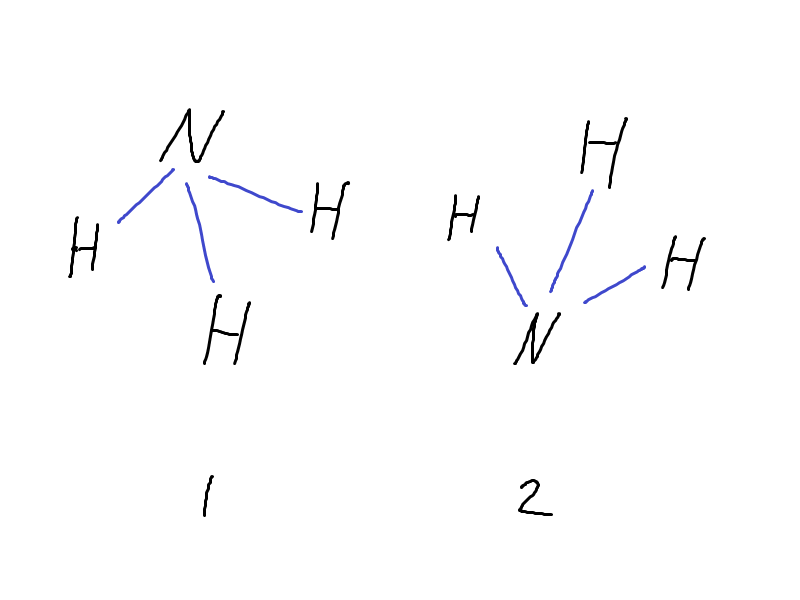
\includegraphics[scale=0.5]{fig/ammonia.png}
\caption{活泼可爱的氨分子}
\label{fig-ammonia}
\end{figure}

简单起见,假设氨分子不能移动或者转动,但是因为一些量子效应,它可以上下翻转。

氨分子的波函数是一个二维矢量:$\mathbf{\psi}=\begin{bmatrix} \psi_1 \\ \psi_2 \end{bmatrix}$。$\psi_1$和$\psi_2$分别表示它处于状态$1$和状态$2$的概率幅,它们都是复数。这里说的概率幅并不是概率,具体待会再讲。

而它的$H$是一个矩阵:$\mathbf{H}=\begin{bmatrix} E_0 & \Delta E \\ \Delta E & E_0 \end{bmatrix}$。$E_0$是氨分子的能量,就是把几根化学键的键能加起来得到的能量。$\Delta E$表示翻转所减少的能量,$\Delta E$越大,翻转就越容易。为什么$H$是这样,也要待会才能明白。

现在来看薛定谔方程:$\rmi \hbar \ppt \mathbf{\psi}=\mathbf{H} \psi$,前面已经知道它的解可以直接写成$\mathbf{\psi}=\rme^{-\rmi \frac{t}{\hbar} \mathbf{H}} \mathbf{\psi_0}$,但是这么写并没有什么用。我们要分别解出$\psi_1$和$\psi_2$关于时间的函数,因此把这个矩阵方程写成两个标量方程:
\begin{align*}
\rmi \hbar \ppt \psi_1&=E_0 \psi_1+\Delta E \psi_2 & \rmi \hbar \ppt \psi_2&=\Delta E \psi_1+E_0 \psi_2
\end{align*}

先把问题再简化一点,假设氨分子连上下翻转的量子效应都没有,也就是$\Delta E=0$,那么
\begin{align*}
\rmi \hbar \ppt \psi_1&=E_0 \psi_1 & \rmi \hbar \ppt \psi_2&=E_0 \psi_2
\end{align*}

可以直接解出$\psi_1=\psi_{1 0} \rme^{-\rmi \frac{E_0}{\hbar} t}$,$\psi_2=\psi_{2 0} \rme^{-\rmi \frac{E_0}{\hbar} t}$,$\psi_{1 0}$和$\psi_{2 0}$是待定的初始条件。

量子力学的另一条基本假设是:我们可以用实验测量一个氨分子在状态$1$还是状态$2$,在某个状态的概率为概率幅的模长的平方。比如在状态$1$的概率$P_1=|\psi_1|^2=\psi_1 \psi_1^*=\psi_{1 0}^2$。$\psi_1$的模长是不变的,所以$P_1$与时间无关,这样的波函数叫作定态。在状态$2$的概率则是$P_2=\psi_{2 0}^2$。既然它是一个概率,那么$P_1+P_2=1$,对初始条件的要求就是$\psi_{1 0}^2+\psi_{2 0}^2=1$。
\section{氨分子振荡;中微子振荡}
只有定态就太无聊了,现在来考虑氨分子的翻转。把上面的方程一加一减,得到
\begin{align*}
\rmi \hbar \ppt (\psi_1+\psi_2)&=(E_0+\Delta E)(\psi_1+\psi_2) & \rmi \hbar \ppt (\psi_1-\psi_2)&=(E_0-\Delta E)(\psi_1-\psi_2)
\end{align*}

可以直接解出$(\psi_1+\psi_2)=(\psi_{1 0}+\psi_{2 0}) \rme^{-\rmi \frac{E_0+\Delta E}{\hbar} t}$,$(\psi_1-\psi_2)=(\psi_{1 0}-\psi_{2 0}) \rme^{-\rmi \frac{E_0-\Delta E}{\hbar} t}$。

不妨设初始时氨分子一定在状态$1$,$\psi_1=1$,$\psi_2=0$。那么
\begin{align*}
\psi_1&=\frac{1}{2}((\psi_{1 0}+\psi_{2 0}) \rme^{-\rmi \frac{E_0+\Delta E}{\hbar} t}+(\psi_{1 0}-\psi_{2 0}) \rme^{-\rmi \frac{E_0-\Delta E}{\hbar} t}) \\
&=\frac{1}{2}(\rme^{-\rmi \frac{E_0+\Delta E}{\hbar} t}+\rme^{-\rmi \frac{E_0-\Delta E}{\hbar} t}) \\
&=\frac{1}{2}(\rme^{-\rmi \frac{\Delta E}{\hbar} t}+\rme^{+\rmi \frac{\Delta E}{\hbar} t}) \rme^{-\rmi \frac{E_0}{\hbar} t} \\
&=\cos (\frac{\Delta E}{\hbar} t) \rme^{-\rmi \frac{E_0}{\hbar} t}
\end{align*}
\begin{figure}[htb]
\centering
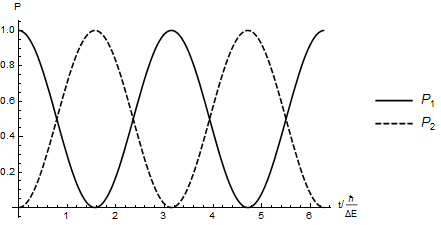
\includegraphics[scale=0.5]{fig/ammonia-osc.png}
\caption{氨分子转起来了}
\label{fig-ammonia-osc}
\end{figure}

同理可得$\psi_2=-\rmi \sin (\frac{\Delta E}{\hbar} t) \rme^{-\rmi \frac{E_0}{\hbar} t}$。$P_1=\cos^2 (\frac{\Delta E}{\hbar} t)$,$P_2=\sin^2 (\frac{\Delta E}{\hbar} t)$,如图\ref{fig-ammonia-osc}。可以看出,随着时间的推移,氨分子在不断翻转,而且始终满足$P_1+P_2=1$。恭喜你!你已经会用量子力学来解决问题了!

$\Delta E$越大,氨分子翻转得越快。翻转一次需要的时间$\tau=\frac{\hbar}{\Delta E}$,它有时间的量纲,至于$2 \pi$之类的系数在这里并不重要。

前几年有一个热门的东西叫中微子振荡。中微子分为三种:电子中微子、$\mu$子中微子、$\tau$子中微子,分别用$\nu_e$、$\nu_\mu$、$\nu_\tau$表示。它们可以互相转化,比如一个$\nu_e$飞着飞着就会变成$\nu_\mu$,原理和上面的氨分子振荡差不多。在$\nu_e$和$\nu_\mu$之间振荡的周期$T=\frac{\hbar}{E_{\nu_\mu}-E_{\nu_e}}$,$E_{\nu_e}$和$E_{\nu_\mu}$分别是$\nu_e$和$\nu_\mu$的能量。

中微子的质量很小,至今都不能确定它是否为零。我们可以测出振荡周期,然后算出中微子的能量,接着算出质量,这是测量中微子质量的方法之一。
\section{能级分裂}
在上面的例子中,如果设$\psi_+=\psi_1+\psi_2$,$\psi_-=\psi_1-\psi_2$,那么它们都是定态:$\psi_+=\psi_{+ 0} \rme^{-\rmi \frac{E_0+\Delta E}{\hbar} t}$,$\psi_-=\psi_{- 0} \rme^{-\rmi \frac{E_0-\Delta E}{\hbar} t}$。

我们可以用实验测量一个氨分子在状态$1$还是状态$2$,也可以用另外的实验测量一个氨分子在状态$+$还是状态$-$。知道了状态$1$和状态$2$的概率幅,就能确定系统的波函数;知道了状态$+$和状态$-$的概率幅,也能确定系统的波函数,相当于选取不同的坐标(专业一点叫\emph{表象})来描述这个系统。

但是状态$+$和状态$-$是什么东西呢?用氨分子的例子可能比较难理解,先看这样一个例子:有两个相同的单摆,用一根弹簧相连,如图\ref{fig-spring-pend}。我们可以让左边的摆单独摆动,也可以让右边的摆单独摆动,分别叫作状态$1$和状态$2$。
\begin{figure}[htb]
\centering
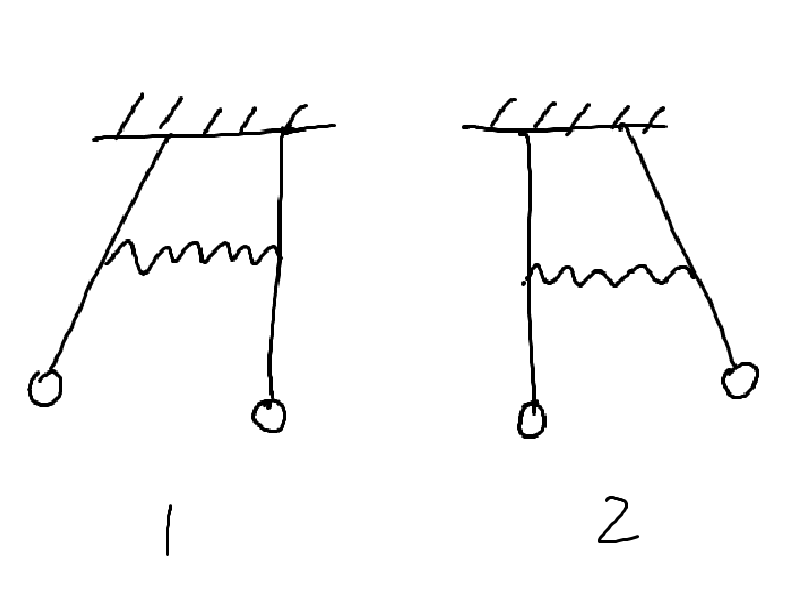
\includegraphics[scale=0.5]{fig/spring-pend.png}
\caption{活泼可爱的弹簧摆}
\label{fig-spring-pend}
\end{figure}

但是我们也可以让两个摆一起摆动,有两种不同的方式,如图\ref{fig-spring-pend-2},相当于刚才的状态$+$和状态$-$。系统的任何运动都可以看作状态$1$和状态$2$的叠加,也可以看作状态$+$和状态$-$的叠加。
\begin{figure}[htb]
\centering
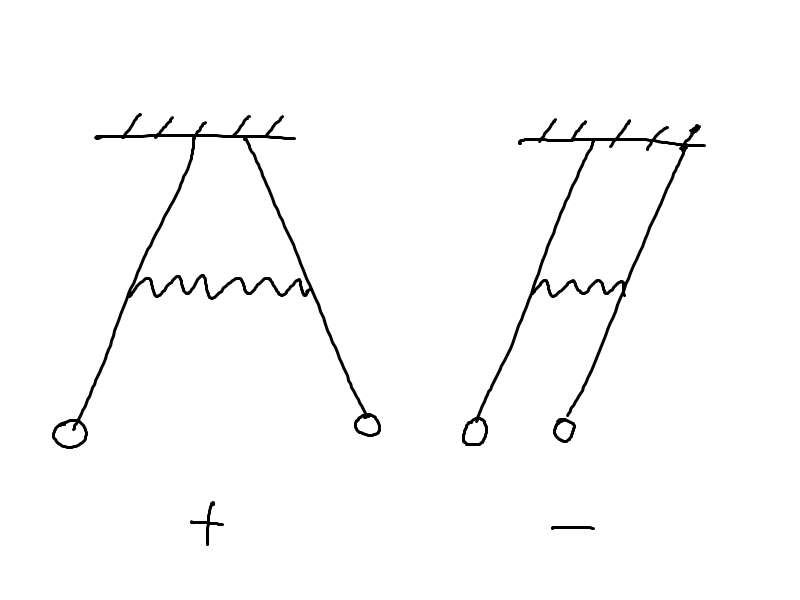
\includegraphics[scale=0.5]{fig/spring-pend-2.png}
\caption{弹簧摆在干奇怪的事情}
\label{fig-spring-pend-2}
\end{figure}

我们还可以选取更加奇怪的坐标来描述这个系统,但是状态$+$和状态$-$有一个好处:它们是定态,或者说它们的运动方程互相独立。学到后面就会发现定态会带来计算上的方便。

回到氨分子的例子,状态$+$的相位是$\rme^{-\rmi \frac{E_0+\Delta E}{\hbar} t}$,而不是$\rme^{-\rmi \frac{E_0}{\hbar} t}$。因此可以认为状态$+$的能量是$E_0+\Delta E$,同理状态$-$的能量是$E_0-\Delta E$。虽然状态$1$和状态$2$的能量是一样的,但是因为它们可以翻转,产生了一个能量较高的状态和一个能量较低的状态,这种现象称为\emph{能级分裂}。

如果考虑一些统计力学的知识,我们还会发现,如果很多氨分子相互作用达到热平衡,会有比较多的氨分子喜欢待在能量较低的状态$-$。(事实上$\frac{P_-}{P_+}=\rme^{\frac{2 \Delta E}{k T}}$,具体的计算非常困难,但是这个结论符合直觉)

高中化学课可能讲过,原子的电子云重叠的时候会出现一条高能量轨道和一条低能量轨道,原理和这个差不多。
\section{一维无限深方势阱}
现在我们把一个粒子装在箱子里。粒子的$\psi$是一个复数,在一维情况下,它是位置和时间的函数$\psi(x,t)$。这里的位置和时间都是连续分布的。(如果不是连续分布的就可以写成矩阵)

粒子的$H=-\frac{\hbar^2}{2 m} \ppxn{2}+V(x)$,其中$-\frac{\hbar^2}{2 m} \ppxn{2}$相当于动能,$V(x)$相当于势能。待会再讲它是怎么来的,现在先用它来算一些有意思的东西。

如果箱子的长度为$a$,$V(x)$可以表示为(分界点的等号不用在意)
\begin{equation*}
V(x)=\begin{cases}
0, &0<x<a \\
\infty, &x<0\text{或}x>a
\end{cases}
\end{equation*}

这样的势能叫作无限深方势阱。$0<x<a$范围内势能为$0$,外面的势能为$\infty$,所以说它是无限深的。从$0$过渡到$\infty$的图像是一条竖直线,所以说它是方的。注意它是一个一维的函数。

现在来解薛定谔方程:
\begin{equation*}
\rmi \hbar \ppt \psi=-\frac{\hbar^2}{2 m} \ppxn{2} \psi+V(x) \psi
\end{equation*}

在势阱里面,$V(x)=0$,这是一个齐次方程。正常的量子力学课本会用分离变量法解这个方程,但是我们只要猜解就行了。我们猜:$\psi=A \rme^{\rmi(k x-\omega t)}$。

($A$仍然是待定的常量。$k$叫作波数,它的量纲与$\frac{1}{x}$相同,不要和弹簧的劲度系数搞混。出于习惯,$\omega$前面有个负号,如果学了相对论会更清楚原因)

代入方程得到$\rmi \hbar \cdot -\rmi \omega \psi=-\frac{\hbar^2}{2 m} \cdot -k^2 \psi$,$\omega=\frac{\hbar k^2}{2 m}$。这就是$\omega$和$k$必须满足的关系。

在势阱外面,无穷大的势能与$\psi$相乘,所以$\psi$必须等于$0$。因此可以把$A$相等,$k$互为相反数的两个解叠加:$\psi=A (\rme^{\rmi(k x-\omega t)}-\rme^{\rmi(-k x-\omega t)})=2 \rmi A \sin(k x) \rme^{-\rmi \omega t}$。它满足边界条件:$x=0$时,$\psi=0$。(如果叠加的时候是$\rme^{\rmi(k x-\omega t)}+\rme^{\rmi(-k x-\omega t)}$,就不满足这个条件)

另一个边界条件是$x=a$时,$\psi=0$,因此$\sin(k a)=0$,$k=\frac{n \pi}{a}(n=1,2,3,\dots)$。(如果$n=0$,$\psi$就恒为$0$,没有物理意义。后面还会发现$n$为负数的情况是没用的)

所以,$\omega=\frac{n^2 \pi^2 \hbar}{2 a^2 m}$,$\psi=A' \sin(\frac{n \pi}{a} x) \rme^{-\rmi \frac{n^2 \pi^2 \hbar}{2 a^2 m} t}$,其中$A'=2 \rmi A$。

这是粒子在时间$t$出现在位置$x$的概率幅,别忘了概率是概率幅的模长的平方:$P=\psi \psi^*=A'^2 \sin^2 (\frac{n \pi}{a} x)=A'^2 \frac{1}{2} (1-\cos(\frac{2 n \pi}{a} x))$。

这个概率必须归一化:$\int_0^a P \opd x=1$(计算这个积分可以用倍角公式),所以$A'=\sqrt{\frac{2}{a}}$,$P=\frac{2}{a} \sin^2 (\frac{n \pi}{a} x)=\frac{1}{a} (1-\cos(\frac{2 n \pi}{a} x))$,这就是粒子位置的概率分布。$n=1,2,3$时,$P(x)$如图\ref{fig-square-well}。
\begin{figure}[htb]
\centering
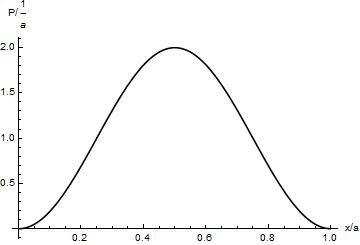
\includegraphics[scale=0.4]{fig/square-well.png}
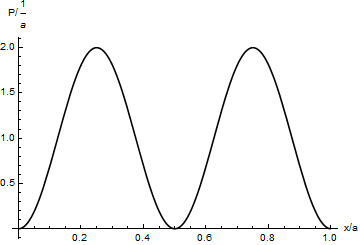
\includegraphics[scale=0.4]{fig/square-well-2.png}
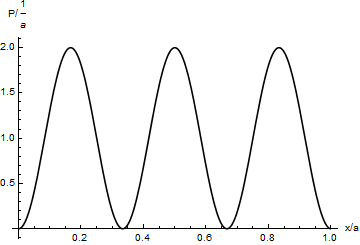
\includegraphics[scale=0.4]{fig/square-well-3.png}
\caption{粒子在方势阱里的位置分布}
\label{fig-square-well}
\end{figure}

前面说过$\rme^{-\rmi \omega t}$中的$\omega=\frac{E}{\hbar}$,所以粒子的能量$E=\hbar \omega=\frac{n^2 \pi^2 \hbar^2}{2 a^2 m}$。我们从小就知道,量子力学当中的能量不能连续变化,只能取不连续的值,这是微分方程的解所要求的。

可以看出,$n$越大,$E$就越大,粒子越容易跑到势阱中的各个地方,而$n$小的时候粒子不容易跑到势阱的边上。$\hbar$是一个很小的量,我们平常接触到的能量对应的$n$很大,所以没有明显的量子效应。

粒子位置的统计平均$\overline{x}=\int_0^a x P(x) \opd x=\frac{a}{2}$(先用倍角公式,然后拆成奇函数和偶函数),这个结果符合直觉。

$\psi$的量纲与$x^{-\frac{1}{2}}$相同,这样才能让$\int_{-\infty}^{\infty} \psi \psi^* \opd x=1$,右边是概率,是一个无量纲的数。现在你可以检查一下上面式子的量纲。在其他问题中,$\psi$的自变量不同,量纲也会不同。
\section{动量;动量算符}
粒子的平均位置$\overline{x}=\int_{-\infty}^{\infty} x \psi \psi^* \opd x$,但是我们一般写成$\int_{-\infty}^{\infty} \psi^* x \psi \opd x$。

粒子的平均速度是什么呢?在波函数中只有位置,没有速度,但是我们可以定义平均速度$\overline{v}=\frac{\opd \overline{x}}{\opd t}$。然后进行一些计算:(前方高能,看不懂可以先跳过)
\begin{align*}
\overline{v}&=\opdt \int_{-\infty}^{\infty} \psi^* x \psi \opd x \\
&=\int_{-\infty}^{\infty} \ppt(\psi^* x \psi) \opd x
\internote{(为什么要把$\opdt$变成$\ppt$呢?如果有一个函数$f(x,t)$,它的全微分$\opd f=\frac{\partial f}{\partial x} \opd x+\frac{\partial f}{\partial t} \opd t$,$\frac{\opd f}{\opd t}=\frac{\partial f}{\partial x} \frac{\opd x}{\opd t}+\frac{\partial f}{\partial t}$。这里$x$和$t$是独立的变量,$\frac{\opd x}{\opd t}=0$。如果$x$与$t$有关,就不能这样了。)}
&=\int_{-\infty}^{\infty} x \psi^* \ppt \psi+x \psi \ppt \psi^* \opd x
\end{align*}

我们要把$\psi^* \ppt \psi+\psi \ppt \psi^*$变成对$x$的微分,然后对$x$积分才方便。按照薛定谔方程:
\begin{align*}
\ppt \psi&=-\frac{\rmi}{\hbar} H \psi \\
&=-\frac{\rmi}{\hbar}(-\frac{\hbar^2}{2 m}\ppxn{2} \psi+V \psi) \\
&=\frac{\rmi \hbar}{2 m} \ppxn{2} \psi-\frac{\rmi}{\hbar} V \psi
\end{align*}

共轭项则是$\ppt \psi^*=-\frac{\rmi \hbar}{2 m} \ppxn{2} \psi^*+\frac{\rmi}{\hbar} V \psi^*$。

所以$\psi^* \ppt \psi+\psi \ppt \psi^*$中含有$V$的项会消掉,剩下$\frac{\rmi \hbar}{2 m}(\psi^* \ppxn{2} \psi-\psi \ppxn{2} \psi^*)$,它还可以写成$\frac{\rmi \hbar}{2 m} \ppx(\psi^* \ppx \psi-\psi \ppx \psi^*)$。

现在可以继续算$\overline{v}$,利用分部积分:
\begin{align*}
\overline{v}&=\frac{\rmi \hbar}{2 m} \int_{-\infty}^{\infty} x \ppx(\psi^* \ppx \psi-\psi \ppx \psi^*) \opd x \\
&=-\frac{\rmi \hbar}{2 m} \int_{-\infty}^{\infty} (\psi^* \ppx \psi-\psi \ppx \psi^*) \opd x \\
&=-\frac{\rmi \hbar}{2 m} \int_{-\infty}^{\infty} (\psi^* \ppx \psi+\psi^* \ppx \psi) \opd x \\
&=\int_{-\infty}^{\infty} \psi^* (-\frac{\rmi \hbar}{m} \ppx) \psi \opd x
\end{align*}

如果定义粒子的平均动量$\overline{p}=m \overline{v}$,那么$\overline{p}=\int_{-\infty}^{\infty} \psi^* (-\rmi \hbar \ppx) \psi \opd x$,就是把平均位置中的$x$换成了$-\rmi \hbar \ppx$。$-\rmi \hbar \ppx$称为动量算符,用$\hat{p}$表示。还可以定义位置算符$\hat{x}$就是$x$。

(量子力学经常研究动量,而不是速度。神奇的是,位置与动量的乘积的量纲与$\hbar$相同。)

如果粒子在位置$x$处的概率为$P(x)=\psi(x) \psi^*(x)$,动量为$p(x)$,那么(对位置的)平均动量就是$\overline{p}=\int_{-\infty}^{\infty} \psi^* p \psi$。然而在量子力学中,我们不能确定粒子在某个位置的动量$p(x)$。如果要计算平均动量,可以对$\hat{p}$“计算平均值”。接下来还会讲确定动量的概率分布的方法。

$\hat{p}$并不是一个函数,前面说过,它是一种把一个函数变成另一个函数的变换操作。只有在它的右边“乘”上一个函数,也就是对这个函数求导,才能得到另一个函数。

现在就知道粒子的$H=-\frac{\hbar^2}{2 m} \ppxn{2}+V$是怎么来的了:在牛顿力学中,动能为$\frac{1}{2} m v^2=\frac{p^2}{2 m}$,如果把$p$换成$\hat{p}$,就是$\frac{\hat{p}^2}{2 m}=-\frac{\hbar^2}{2 m} \ppxn{2}$,这一项代表动能。$V$则代表势能,加起来就是总能量。然而出于习惯,我们用$H$而不是$\hat{E}$表示能量,把它叫作哈密顿算符。

刚才算出了粒子在一维无限深方势阱中的定态波函数:
\begin{equation*}
\psi=\sqrt{\frac{2}{a}} \sin(\frac{n \pi}{a} x) \rme^{-\rmi \frac{n^2 \pi^2 \hbar}{2 a^2 m} t}, 0<x<a
\end{equation*}

现在我们假装认真地算一下它的平均动量:
\begin{align*}
\ppx \psi&=\frac{n \pi}{a} \sqrt{\frac{2}{a}} \cos(\frac{n \pi}{a} x) \rme^{-\rmi \frac{n^2 \pi^2 \hbar}{2 a^2 m} t} \\
\psi^* (-\rmi \hbar \ppx) \psi&=-\frac{2 \rmi n \pi \hbar}{a^2} \sin(\frac{n \pi}{a} x) \cos(\frac{n \pi}{a} x) \\
&=-\frac{\rmi n \pi \hbar}{a^2} \sin(\frac{2 n \pi}{a} x) \\
\overline{p}&=\int_{0}^{a} \psi^* (-\rmi \hbar \ppx) \psi \opd x \\
&=-\frac{\rmi \hbar}{2 a}(1-\cos(2 n \pi)) \\
&=0
\end{align*}

上面已经算过$\overline{x}=\frac{a}{2}$,与$x$无关,其实可以直接知道$\overline{p}=m \frac{\opd \overline{x}}{\opd t}=0$。

(这个定态的栗子好像举得很无聊,然而不是定态的话有很大的计算量)
\section{动量与傅立叶变换}
(因为章节安排的一些问题,这一节要看过后面的傅立叶变换才能看)

在讲氨分子的时候,可以用状态$1$和$2$描述氨分子的状态,也可以用状态$+$和$-$来描述,这两种方法相当于不同的坐标系,专业一点叫\emph{表象}。刚才用位置和时间描述粒子的状态,现在还可以用动量和时间来描述,也就是把位置表象下的波函数$\psi(x,t)$变换成动量表象下的波函数$\phi(p,t)$。($\psi$和$\phi$这两个字母容易搞混,但是很多人都在这么写)

$\psi(x,t)$可以分解为简谐波$\rme^{\rmi(k x-\omega t)}=\rme^{\rmi k x} \rme^{-\rmi \omega t}$(先不管振幅),$k$是波数,动量$p=\hbar k$。也就是说,动量表象就是位置表象的频谱,再乘上一些系数$\hbar$,而时间的部分不用变。

($p=\hbar k$和$E=\hbar \omega$这两个公式看起来很对称,高中学的应该是$p=\frac{h c}{\lambda}$和$E=h \nu$)

傅立叶变换的公式是:
\begin{align*}
g(k)&=\mathscr{F}_{x \rightarrow k} f(x)=\frac{1}{\sqrt{2 \pi}} \int_{-\infty}^{\infty} f(x) \rme^{-\rmi k x} \opd x &
f(x)&=\mathscr{F}^{-1}_{x \rightarrow k} g(k)=\frac{1}{\sqrt{2 \pi}} \int_{-\infty}^{\infty} g(k) \rme^{\rmi k x} \opd k
\end{align*}

乘上一些$\hbar$(可以通过换元,也可以凑量纲),就得到表象变换的公式:
\begin{align*}
\phi(p,t)&=\sqrt{\hbar} \mathscr{F}_{x \rightarrow \frac{p}{\hbar}} \psi(x,t) & \psi(x,t)&=\frac{1}{\sqrt{\hbar}} \mathscr{F}^{-1}_{x \rightarrow \frac{p}{\hbar}} \phi(p,t) \\
&=\frac{1}{\sqrt{2 \pi \hbar}} \int_{-\infty}^{\infty} \psi(x,t) \rme^{-\frac{\rmi}{\hbar} p x} \opd x & &=\frac{1}{\sqrt{2 \pi \hbar}} \int_{-\infty}^{\infty} \phi(p,t) \rme^{\frac{\rmi}{\hbar} p x} \opd p
\end{align*}

如果$\psi$已经归一化,那么$\phi$仍然是归一化的:$\int_{-\infty}^{\infty} \phi \phi^* \opd p=1$。粒子动量为$p$的概率$P=\phi \phi^*$。别忘了$\psi(x,t)$的量纲与$x^{-\frac{1}{2}}$相同,而$\phi(p,t)$的量纲与$p^{-\frac{1}{2}}$相同。

我们把这个公式凑出来了,然而具体的计算是很困难的。比如刚才的波函数:
\begin{equation*}
\psi=\sqrt{\frac{2}{a}} \sin(\frac{n \pi}{a} x) \rme^{-\rmi \frac{n^2 \pi^2 \hbar}{2 a^2 m} t}, 0<x<a
\end{equation*}

可以算出:(啊。。我想不出简单的栗子,只好硬着头皮讲下去了)
\begin{align*}
\phi=&\frac{1}{\sqrt{2 \pi \hbar}} \int_{-\infty}^{\infty} \psi \rme^{-\frac{\rmi}{\hbar} p x} \opd x \\
&=\sqrt{\frac{a}{2 \hbar}} \frac{n (1-(-1)^n \rme^{-\rmi \frac{a p}{\hbar}})}{(n \pi)^2-(\frac{a p}{\hbar})^2} \\
P&=\phi \phi^* \\
&=\frac{a}{\hbar} \frac{2 n^2 \cos^2 \frac{a p}{2 \hbar}}{((n \pi)^2-(\frac{a p}{\hbar})^2)^2}
\end{align*}

$n=1,4,7$时,$P(p)$如图\ref{fig-square-well-p}。可以看出,动量的概率是偶函数,平均值确实为$0$。如果$\psi$是简谐波,变换之后的$\phi$就是两个峰,而且是无限高、无限细的$\delta$函数;但是$\psi$有$0<x<a$的范围限制,所以$\phi$是两个有一定高度和宽度的峰($n=1$时合并为一个),旁边还有一些小峰。$n$越大,峰位置的绝对值越大,说明粒子动得越厉害。
\begin{figure}[htb]
\centering
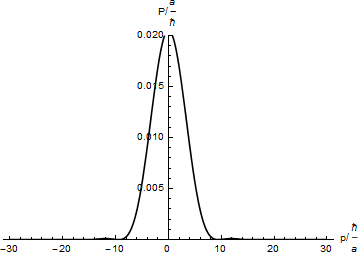
\includegraphics[scale=0.4]{fig/square-well-p.png}
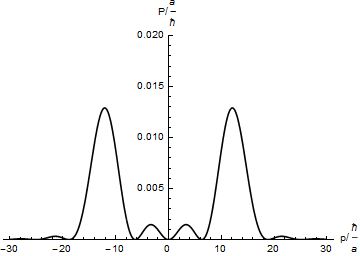
\includegraphics[scale=0.4]{fig/square-well-p-4.png}
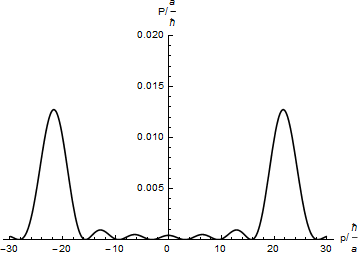
\includegraphics[scale=0.4]{fig/square-well-p-7.png}
\caption{粒子在方势阱里的动量分布}
\label{fig-square-well-p}
\end{figure}

算符在不同的表象下也有不同的样子。动量表象下的动量算符$\hat{p}$就是$p$,而位置算符$\hat{x}=\rmi \hbar \ppp$(注意这里没有负号,推导过程和刚才差不多)。想要在动量表象下计算平均位置,仍然可以对$\hat{x}$“计算平均值”:$\overline{x}=\int_{-\infty}^{\infty} \phi^* \hat{x} \phi \opd p$。

刚才推导位置表象下的动量算符用到了薛定谔方程。如果不知道薛定谔方程,利用傅立叶变换也可以推导:
\begin{align*}
\overline{p}&=\int_{-\infty}^{\infty} \phi^* p \phi \opd p \\
&=\frac{1}{\sqrt{2 \pi \hbar}} \int_{-\infty}^{\infty} \int_{-\infty}^{\infty} \psi^* \rme^{\frac{\rmi}{\hbar} p x} \opd x p \phi \opd p \\
&=\frac{1}{\sqrt{2 \pi \hbar}} \int_{-\infty}^{\infty} \int_{-\infty}^{\infty} \psi^* (-\rmi \hbar \ppx) \rme^{\frac{\rmi}{\hbar} p x} \opd x \phi \opd p \\
&=\int_{-\infty}^{\infty} \psi^* (-\rmi \hbar \ppx) \frac{1}{\sqrt{2 \pi \hbar}} \int_{-\infty}^{\infty} \phi \rme^{\frac{\rmi}{\hbar} p x} \opd p \opd x \\
&=\int_{-\infty}^{\infty} \psi^* (-\rmi \hbar \ppx) \psi \opd x
\end{align*}

在简谐波的表达式$\rme^{\rmi(k x-\omega t)}$中,位置和时间看起来是对称的(相差一个负号),动量和能量也是对称的。既然$\hat{p}=-\rmi \hbar \ppx$,那么$\hat{E}=\rmi \hbar \ppt$(相差一个负号),这就是薛定谔方程。
